\documentclass[sigconf,natbib=true,anonymous=true]{acmart}
\settopmatter{printacmref=false}
\setcopyright{none}
\renewcommand\footnotetextcopyrightpermission[1]{}
% Track: full papers. The session-27 brief (BRIEF.md) sends this version to the full-paper track if H27a and H27b
% both survive under E1, and to the reproducibility or resource track otherwise. Both survived (results/session27.md).
\acmConference[SIGIR '27]{Submitted to the full-paper track of the 50th International ACM SIGIR Conference on Research and Development in Information Retrieval}{July 2027}{San Jose, CA, USA}
\usepackage{booktabs}
\usepackage{multirow}

\newcommand{\rep}[1]{\texttt{#1}}
\newcommand{\ci}[2]{[\ensuremath{#1},\,\ensuremath{#2}]}  % math minus signs in intervals
\newcommand{\anonrepo}{the anonymised repository (link given with the submission)}
\setlength{\emergencystretch}{2em}

\begin{document}

\title{A Few Vectors for a Mixed Folder: A Pre-Registered Measurement of Pooled Directory Embeddings}

\author{Anonymous Author(s)}
\affiliation{\institution{Anonymous Institution}\country{}}

\begin{abstract}
A folder's metadata is read before its files and holds a few kilobytes. A vector stored there can route a query without opening the folder, and the cheapest is the mean of its files' embeddings. We ask when the mean is enough and what to store when it is not. Under our main vision-language embedder, the mean does at least as well as a few representatives on GitHub directories that do not mix media, about 95 percent of those eligible. Representatives for mixed folders only are level with the mean over all directories (both post hoc). Where a folder mixes images and texts, the mean loses its minority modality. On Zenodo record folders a held-out minority file finds its folder 0.16 to 0.25 recall@5 less often with the mean than with a few per-modality representatives under two vision-language embedders, and 0.35 to 0.50 less often under two CLIP-family dual towers. There, four representatives per label are not inferior to searching every file, at a 0.02 margin, over all queries and in every cell under all four encoders (post hoc). On queries that a language model wrote as a simulated searcher, the loss under the main embedder is 0.14 (interval 0.02 to 0.28) for pictures in text-heavy folders and 0.42 (0.28 to 0.56) for documents in image-heavy ones. At three per label every folder's representatives fit in 8 KiB at a further cost of at most 0.012 in any cell. In 2 KiB a per-kind sample of the folder's files keeps the minority files the mean loses, and on ext4 a summary of 2,048 or 4,000 bytes costs 1.2 blocks per cold directory read. With every creator weighted equally the main embedder's file-query loss is 0.13 and 0.14, and 0.06 and 0.12 on queries whose names do not give the folder away. Every hypothesis was fixed in a brief before its test. Five briefs are timestamped externally, the rest dated by the working repository's history. Code, manifests and briefs are released.
\end{abstract}

\begin{CCSXML}
<ccs2012>
<concept><concept_id>10002951.10003317.10003371.10003386</concept_id>
<concept_desc>Information systems~Multimedia and multimodal retrieval</concept_desc>
<concept_significance>500</concept_significance></concept>
<concept><concept_id>10002951.10003317.10003338</concept_id>
<concept_desc>Information systems~Retrieval models and ranking</concept_desc>
<concept_significance>300</concept_significance></concept>
</ccs2012>
\end{CCSXML}
\ccsdesc[500]{Information systems~Multimedia and multimodal retrieval}
\ccsdesc[300]{Information systems~Retrieval models and ranking}
\keywords{modality gap, collection representation, directory retrieval, multimodal embeddings, pre-registration}

\maketitle

\section{Introduction}
\label{sec:intro}

A file system reaches a folder before it reaches the folder's files. A folder's own metadata can be read without listing or opening anything inside it, but it holds little. An extended attribute holds at most 64 KiB on Linux, and ext4 and APFS keep a value with the directory's own record only up to about 4 KB \citep{linux2026xattr,e2fsprogs2025ext4,apple2020apfs}. A vector kept there can be read before a search decides whether to open the folder, and it has to fit in a fixed number of bytes. Searching every file needs the vector of every file, which such a search has not yet read, so we treat file-level search as the reference and ask how much of it a few kilobytes on the folder keep.

Folders are becoming units of retrieval again. Retrieval-augmented generation can route a query to a source before it searches inside it, and one router for text sources takes the centroid of each source's document embeddings as an input \citep{dhasade2026ragroute}. A context database for agents organises resources, memories and skills as a directory tree whose directories carry a short abstract used for vector retrieval \citep{openviking2026docs}. The cheapest representation of a container in an embedding space is the mean of its members' vectors.

Many containers mix media. A record of a field study holds photographs, a scanned permit, a spreadsheet of readings and a README, and a software repository holds screenshots beside its code. Several embedders put such files in one space \citep{gunther2025jinav4,koukounas2024jinaclipv2,zhang2025gme,nussbaum2024nomicvision}. In contrastive models, image and text embeddings occupy offset regions of that space \citep{liang2022mindgap}, and in mixed-modality retrieval the offset biases ranking toward the query's own modality \citep{li2025grclip}. That one mean misrepresents a group made of two clusters is expected, and textbook material for classifiers \citep{manning2008iir}. We found no measurement of how much a pooled vector loses on real mixed-media folders, or of what a folder's few kilobytes can keep instead.

We measure both on two sources, Zenodo record folders and directories of public GitHub repositories, under four encoders from three vendors, and on queries that a language model wrote as a simulated searcher. Each test was registered with its criterion before it ran (Table~\ref{tab:verdicts}). We report four findings.

\begin{enumerate}
\item \textbf{Where a folder does not mix media, the mean does as well as a few representatives.} Mixed directories are 4 to 5 percent of eligible GitHub directories, and on the others the mean does at least as well under the first embedder (post hoc). Keeping representatives only for folders that hold an image and another file keeps most of the minority gain at the natural mix and is level with the mean over all directories (Section~\ref{sec:github}, post hoc). On whole repository trees the mean is the better summary for inner nodes over all queries (Section~\ref{sec:tree}).
\item \textbf{Where it mixes, the mean misses the minority files.} On Zenodo the loss is 0.16 to 0.25 recall@5 under two vision-language embedders and 0.35 to 0.50 under two CLIP-family dual towers (Section~\ref{sec:loss}). It is smaller with creators weighted equally, 0.13 and 0.14 under the first embedder, and it holds at about half its size on image queries whose file names do not give the folder away, where creators weighted equally give 0.06 and 0.12. On GitHub it is 0.21 and 0.20 for files with a sibling of their kind (Section~\ref{sec:github}).
\item \textbf{The loss reaches queries written by a simulated searcher.} A language model wrote queries as a simulated searcher for 100 Zenodo folders, from what a person would see of them. On those queries the loss under the first embedder is 0.14 for pictures in text-heavy folders and 0.42 for documents in image-heavy ones, and both registered tests passed (Section~\ref{sec:searcher}). Under E2 the picture cell shows no loss. No person wrote queries for this study.
\item \textbf{A few representatives per kind fix it, within a folder's bytes.} A mixed folder is two clusters, and centering, 40 single-vector variants and a folder abstract written by a model fall short on the minority files (Sections~\ref{sec:mechanism}, \ref{sec:abstracts} and~\ref{sec:remedy}). On the confirmation set four $k$-means centroids per file type are not inferior to searching every file in every cell under all four encoders (post hoc), and every folder's three per type fit in 8 KiB at a further cost of at most 0.012 in any cell (Section~\ref{sec:remedy}). File type is a cheap way to split the budget, and from three per type up blind clustering at the same count is within 0.015 of it in every cell (Section~\ref{sec:hetero}).
\end{enumerate}

The contribution is a measurement with its controls and the rule it supports, and the remedies we test are existing ones. The briefs, results, manifests and code are in \anonrepo.

\section{Related work}
\label{sec:related}

\paragraph{The modality gap.} \citet{liang2022mindgap} showed that multi-modal contrastive models embed images and text in separate regions of their shared space. For mixed-modality search, \citet{li2025grclip} show that documents of the query's modality are ranked higher and remove the bias by subtracting each modality's mean embedding (GR-CLIP). Each of their documents is a single image and a single text segment, and they name multi-image, multi-text documents as future work. \citet{liu2026geometry} report, for CLIP-style models, that mean-centering removes the offset between the modality centroids and leaves what they call the distribution gap unchanged. For one item with several modality streams, \citet{mehrish2026centroid} report that symmetric aggregators often lag the strongest single stream. The closest work to a pooled representation is \citet{grassucci2026closing}, who consider the centroid of a semantic class that spans two modalities and show that closing the gap with a training objective improves clustering while leaving retrieval rankings mostly unaffected. These works study single items, or a class centroid under a training objective. None pools the embeddings of a folder's files, of different modalities and different content, into one vector of a frozen encoder.

\paragraph{Representing a collection.} Federated search has two families of collection representation \citep{shokouhi2011federated}. Lexicon-based methods such as CORI treat a collection as one large bag of words \citep{callan1995cori}, and document-surrogate methods such as ReDDE select collections through sampled documents \citep{si2003redde}. Whether one summary or several members should stand for a collection has been asked before, in text. For blog site search, \citet{seo2008blogsite} found that selection through clusters of highly ranked postings outperformed a global representation of the blog. In expert finding, \citet{balog2006expert} found that ranking documents first and aggregating them per candidate outperformed one representation per candidate in nearly all settings. Dense routers have returned to the single summary \citep{dhasade2026ragroute,lee2025routerretriever}, and \citet{lee2025routerretriever} report that additional centroids per group act as distractors. Cluster-based retrieval asks the same question of a cluster: the cluster hypothesis \citep{voorhees1985cluster} holds that documents in one cluster answer the same queries, and cluster-based retrieval with language models ranks a cluster by one model of its documents \citep{liu2004cluster,kurland2004corpus}. A folder is such a cluster, one the file system already provides. All of these collections are text. This paper adds the modality axis.

\paragraph{Multiple representatives.} That one centroid fails a class made of several clusters is textbook material. A nearest-centroid classifier misclassifies such a class \citep{manning2008iir}, and prototype methods, several representatives per class, are a standard chapter of statistical learning \citep{hastie2009esl}. The capacity of a single dense vector has also been studied for text retrieval \citep{luan2021sparse}. The loss measured here is therefore expected in kind, and what this paper adds is its size on real mixed-media folders and what fits in the bytes a folder offers. Recommendation has long represented one entity by several vectors, scored by the maximum over a user's interests \citep{weston2013maxmf}, extracted by capsule routing \citep{li2019mind} or kept as cluster medoids \citep{pal2020pinnersage}. Late-interaction retrieval keeps every token vector of a passage and scores a query by the sum over its tokens of the best match \citep{khattab2020colbert}. The flat walk is its analogue at file level. No late-interaction encoder was measured here. Pooling the members' vectors before scoring and taking the best member score after it are the early and the late fusion of multimedia analysis \citep{snoek2005fusion}.

\paragraph{Documents, hierarchies and file systems.} Visual document retrieval embeds a page or a screenshot \citep{faysse2025colpali,ma2024dse,yu2025visrag}. One level up, \citet{you2026docpc} compose a document from its pages and report that, among independent page scores, the maximum over pages beats their average, the same direction as our result for folders. Above the document, hierarchical retrieval has so far meant text summaries. RAPTOR clusters text chunks, summarises each cluster with a language model and embeds the summaries \citep{sarthi2024raptor}, and GraphRAG summarises the communities of an entity graph the same way \citep{edge2024graphrag}. OpenViking builds a directory's abstract bottom-up from summaries of its files, turning images and other media into text summaries first \citep{openviking2026docs}. Section~\ref{sec:abstracts} measures a folder abstract built in this way. Semantic file systems attach attributes to files and directories \citep{gifford1991sfs}, and VectorVFS stores an embedding in each file's extended attributes \citep{perone2025vectorvfs}. The same mechanism on a directory would hold the folder's own vectors. The directory-aware vector database of \citet{wang2026directoryaware} treats a directory as a scope predicate on a vector search and has no directory vector. We know of no published work that embeds a mixed-media folder as an object and measures what the embedding retrieves.

\section{Study design}
\label{sec:design}

\paragraph{Corpora.} We use Zenodo records as folders. The pool is the Zenodo search for public records of 3 to 60 files that hold both an image type and a document type under a CC0 or CC-BY licence, 2017 to 2026. We keep files of five kinds (image, PDF, text, table, office document), each at most 25 MB and at most 100 MB per record, and only the newest version of a concept. Four disjoint draws took part (Table~\ref{tab:corpora}). The pilot is 400 directories stratified by image fraction. The retest set is 400 more, drawn the same way with the pilot excluded. The main set holds the 2,808 eligible records the pool had left that could still be downloaded, and the confirmation set holds the 2,597 eligible records of a new pool snapshot, with every earlier record and concept excluded. Images are mostly scientific figures (plots, maps, micrographs) rather than photographs. Two draws of GitHub directories, G1 and G2, and a set of whole repository trees are described in Sections~\ref{sec:github} and~\ref{sec:tree}. Modality labels come from the file: image, pdf\_text, pdf\_scanned (fewer than 50 extracted characters per page), text, table, other (office documents). A directory's image fraction is the share of its files labelled image.

\begin{table}[t]
\caption{The draws of single folders, four of Zenodo records and two of GitHub directories. Directories per image-fraction bucket $[0,.2)$, $[.2,.5)$, $[.5,.8)$, $[.8,1]$; queries are leave-one-out files with a vector, after deduplication.}
\label{tab:corpora}
\setlength{\tabcolsep}{3pt}
\resizebox{\columnwidth}{!}{%
\begin{tabular}{lrrrrr}
\toprule
Draw & Dirs & Files & Size & Per bucket & Queries \\
\midrule
Zenodo pilot & 400 & 4,773 & 5.2 GB & 103/100/98/99 & 4,071 \\
Zenodo retest & 400 & 4,891 & 4.8 GB & 103/99/99/99 & 4,041 \\
Zenodo main & 2,808 & 27,545 & 29.0 GB & 459/1,005/1,034/310 & 23,130 \\
Zenodo confirmation & 2,597 & 25,990 & 28.5 GB & 420/795/978/404 & 21,225 \\
GitHub G1 & 1,600 & 12,656 & 1.6 GB & 700/378/244/278 & 9,089 \\
GitHub G2 & 2,600 & 21,854 & 3.5 GB & 943/772/510/375 & 16,185 \\
\bottomrule
\end{tabular}}
\end{table}

\paragraph{Ground truth.} The task is directory retrieval. For a query file $f$ in a directory $D$ of at least three files, the one relevant item is $D$, and every directory representation is built leaving $f$ out, a simulated known-item query, as used in IR evaluation \citep{azzopardi2007simulated} and for desktop search \citep{kim2009pseudodesktop}. Near-duplicates are found first (exact hash, perceptual hash for images, simhash for text). A file with a near-duplicate anywhere in the set is not a query, because a copy left behind in the directory would make leave-one-out trivial and a copy elsewhere would make it wrong. Recall@$k$ is the fraction of queries whose directory is in the top $k$ of all directories in the set. We report recall@5, with 95 percent paired bootstrap intervals from 1,000 resamples of directories.

\paragraph{Cells.} Queries are grouped by their modality and by the image fraction of their directory. The two \emph{minority} cells are P1, image queries in directories with image fraction below 0.5, and P2, text-like queries (text, table, pdf\_text, other) in directories with image fraction of 0.5 or more. The two \emph{majority} cells M1 and M2 are the complements (image queries in image-heavy directories, text-like queries in text-heavy ones). Scanned PDFs as queries belong to none of the four cells (192 of the 17,140 evaluation queries of the confirmation set).

\paragraph{Encoders.} E1 is jina-embeddings-v4 \citep{gunther2025jinav4}, a Qwen2.5-VL-based embedder with one space for text and images (2,048 dimensions, single-vector mode). E2 is jina-clip-v2 \citep{koukounas2024jinaclipv2}, a CLIP-family dual tower with an 8k-token text side (1,024 dimensions). E3 is gme-Qwen2-VL-2B-Instruct \citep{zhang2025gme}, a unified embedder from another vendor (Alibaba), built on Qwen2-VL-2B (1,536 dimensions). E4 is Nomic Embed v1.5 \citep{nussbaum2024nomicvision,nussbaum2024nomicembed}, a second CLIP-family dual tower, from a third vendor (Nomic AI, 768 dimensions); its texts, files and queries alike, carry the prefix its model card gives for text searched against images, a choice fixed before any E4 number was read. On a pilot check in 20 directories of the confirmation set (text or table file to own-directory image), the median rank is 26 of 159 under E1, 51 under E2, 21 under E3 and 65.5 under E4, against 80 at random, so both towers pass it weakly. Each encoder reads an image as the image itself, at most 602,112 pixels under E1 and E3. E2 and E4 apply their own shipped preprocessing. Text, table, pdf\_text and office documents give the first 2,000 tokens of extracted text, counted by E1's tokenizer for every encoder, and a scanned PDF gives the mean of the vectors of its first eight page renders. On the confirmation set all four embed the same 25,637 of its 25,990 files.

\paragraph{Directory representations.} All are built leave-one-out from the directory's remaining file vectors and scored by the maximum cosine over the directory's vectors. \rep{a} is the pooled centroid, one vector, the mean of the child vectors. \rep{c} runs per-modality $k$-means with $k = \min(3, n_m)$ representatives for a label with $n_m$ files (up to 18; 5.2 to 5.4 on the Zenodo sets), with ten initialisations and one fixed seed. The budget of three was fixed before the first test, and Section~\ref{sec:remedy} varies it. Across three seeds the recall@5 of \rep{c} moves by at most 0.0026 in any cell under any encoder (post hoc). \rep{d} keeps every child vector, the flat file-level walk. It needs the vector of every file and is the reference the compact representations are measured against. Centered variants (\rep{ac}, \rep{cc}, \rep{dc}) subtract from every file vector, and from the query, the mean vector of its own input group (image inputs: image and pdf\_scanned; text inputs: the rest) and renormalise before any pooling, as GR-CLIP does \citep{li2025grclip}. The group means are computed on a 20 percent calibration split of the set's directories, and nothing fitted or chosen on a split is tested on its file queries. Two-vector variants are \rep{bc2}, one centered centroid per input group, and \rep{tb2c}, two centered clusters found by label-blind $k$-means.

\paragraph{Protocol.} The study ran as working sessions in which the authors directed an AI coding assistant. ``Agent'' below means such an assistant. Each test was written into a brief with its criterion before the numbers that decide it were computed, and the results report the verdict either way (Table~\ref{tab:verdicts}). Choices such as an alignment weight were made on the calibration split and tested on the rest. The briefs of the two GitHub draws, the 2 KiB and tree studies and the searcher-query and budget studies were also timestamped with OpenTimestamps \citep{todd2016opentimestamps} before their numbers existed. The earlier briefs, among them those of the other Zenodo tests, and those written after the first round of review, are dated by the history of the working repository alone, which is available on request. Their pre-registration rests on that history. The confirmation set served several studies in turn, and each later brief was written with the earlier results on that set known. One registered result, that no single vector reaches \rep{c} (Section~\ref{sec:remedy}), was re-run after a scoring error had scored the weighted single vectors too low, and it held. We read a compact representation as no worse than \rep{d} when the lower end of the 95 percent interval of their difference is at or above $-0.02$. Analyses added after that review are marked post hoc. Four of them were registered with their criteria before they ran, on draws the study had already read, and Table~\ref{tab:verdicts} marks them. The searcher queries and the budget study were registered after a later round of review, the budget study on a set the study had already read, and we mark it post hoc.

\begin{table*}[t]
\caption{The registered tests and their verdicts, each written with its criterion before it ran. Main and confirmation are Zenodo sets, G1 and G2 GitHub draws. On GitHub a loss is confirmed when the lower end of its interval is at least $+0.05$ with 100 owners or more, and inconclusive with fewer owners. A dagger marks the four tests registered after an earlier round of review, on draws already read. Mixed-only: \rep{c} for folders that hold an image and another file, \rep{a} for the rest.}
\label{tab:verdicts}
\footnotesize
\setlength{\tabcolsep}{3pt}
\begin{tabular}{lll|lll}
\toprule
Test & Data & Verdict & Test & Data & Verdict \\
\midrule
Loss in P1 and P2 & retest, E1 & survived & Creator-clustered interval above zero & confirm., E1 to E4 & survived \\
Loss in P1 and P2 & confirm., E2, E3, E4 & survived & Loss on clean queries at least $+0.05$ & confirm., E1, E3 & survived \\
Loss under E4 above loss under E1 & confirm. & survived & Second implementation, same ranks & confirm., E1 & survived \\
Second calibration seed, same verdicts & confirm., E1, E2 & survived & Abstract against \rep{c} on titles & confirm., E1, E3 & split \\
Centering recovers half of \rep{c}'s gain & main, E1 & died & \rep{c} above abstract, image descriptions & confirm., E1 & survived \\
Labels beat blind $k$-means at equal size & main, E1 & died & Loss in P1s and P2s & G1; G2, E1 & inconcl.; confirmed \\
No single vector within 0.02 of \rep{c} & main, E1 & survived & \rep{c} against \rep{d}, compressed folders & G1, G2 & not inferior \\
Cross-modal guests lose more & main, 10 hosts & survived & Loss on commit subjects & G1; G2 & inconcl.; confirmed \\
Two blind clusters within 0.02 of \rep{c} & confirm. & E1 survived, E2 died & 2 KiB: kind sample above mean & G1; G2, pooled & inconcl.; confirmed \\
Loss on titles of image-heavy folders & confirm., E1 & survived & 2 KiB: kind sample against $k$-means & G1, G2 & inferior \\
\rep{c} against \rep{d}, registered rule & confirm., E3, E4 & survived (not a non-inferiority rule) & 2 KiB: kinds above uniform sample & G1; G2, pooled & inconcl.; kinds matter \\
\rep{c} at one byte against \rep{d} & confirm., E1 to E4 & survived & Walk: kind sample above mean & trees & inconclusive \\
\rep{c} at one bit against \rep{d} & confirm., E1 to E4 & E1, E3 survived & Walk: kinds above uniform sample & trees & kinds matter \\
\rep{c} at one bit above \rep{a} (float32) & confirm., E1 to E4 & survived & Walk against flat read & trees & inferior \\
Loss with file names fused$^\dagger$ & confirm., E1, E3 & survived & Mixed-only not below \rep{a}, all$^\dagger$ & G1+G2, natural mix & not inferior \\
Mixed-only: loss in P1s, P2s$^\dagger$ & G1+G2, natural mix & confirmed & Mixed-only above \rep{c}, all$^\dagger$ & G1+G2, natural mix & died \\
Searcher queries: loss, pictures and documents & confirm., E1 & survived & Searcher queries: \rep{c} against \rep{d} & confirm., E1 & not inferior \\
\bottomrule
\end{tabular}
\end{table*}

\section{The pooled vector misses the minority files}
\label{sec:loss}

On the pilot set the pooled centroid lost 0.27 recall@5 against \rep{c} on image queries in the most text-heavy directories and 0.27 on text-like queries in the most image-heavy ones, and almost nothing where the query's modality dominated its directory. We registered this as a test with its cells and kill rule (dead unless the interval of \rep{c} minus \rep{a} excludes zero in both minority cells) and ran it on the retest set. It survived, with \rep{c} minus \rep{a} at $+0.179$ \ci{+0.115}{+0.251} in P1 and $+0.200$ \ci{+0.135}{+0.270} in P2. On the main set the loss is $+0.238$ \ci{+0.207}{+0.268} and $+0.233$ \ci{+0.207}{+0.262}. On the confirmation set under E1 it is $+0.253$ \ci{+0.214}{+0.294} and $+0.169$ \ci{+0.136}{+0.200}; these two rows are reported rather than registered tests, and the registered tests on the confirmation set are the other encoders, a second calibration seed and the checks of Section~\ref{sec:validity}. Figure~\ref{fig:loss} collects the six measurements, and Table~\ref{tab:cells} gives the cells of the confirmation set.

\begin{figure}[t]
\centering
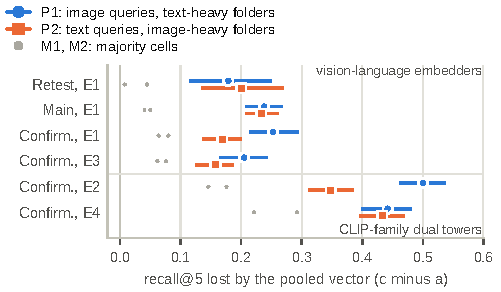
\includegraphics[width=\columnwidth]{fig_loss_col.pdf}
\caption{How much the pooled vector loses: recall@5 of \rep{c} minus \rep{a} with paired 95 percent intervals, on the retest, main and confirmation sets under E1 and on the confirmation set under E2, E3 and E4. Gray: the majority cells (M1, M2).}
\label{fig:loss}
\end{figure}

\begin{table}[t]
\caption{Recall@5 on the confirmation set's evaluation split (17,140 queries over 2,035 directories, 2,597 ranked) by encoder, representation and cell. The cells hold 1,959 (P1), 2,146 (P2), 5,571 (M1) and 7,272 (M2) queries. Vectors per directory in parentheses. File names: a router on file names alone, no encoder.}
\label{tab:cells}
\setlength{\tabcolsep}{4.2pt}
\small
\begin{tabular}{lrrrrr}
\toprule
 & all & P1 & P2 & M1 & M2 \\
\midrule
\multicolumn{6}{l}{E1 jina-embeddings-v4} \\
\rep{a} (1.00) & 0.692 & 0.421 & 0.370 & 0.730 & 0.830 \\
\rep{ac} (1.00) & 0.719 & 0.513 & 0.474 & 0.734 & 0.835 \\
\rep{bc2} (1.95) & 0.769 & 0.671 & 0.591 & 0.773 & 0.845 \\
\rep{tb2c} (2.00) & 0.781 & 0.638 & 0.575 & 0.805 & 0.862 \\
\rep{c} (5.20) & 0.796 & 0.674 & 0.539 & 0.810 & 0.894 \\
\rep{cc} (5.20) & 0.810 & 0.713 & 0.590 & 0.814 & 0.899 \\
\rep{d} (9.87) & 0.804 & 0.685 & 0.551 & 0.821 & 0.897 \\
\rep{dc} (9.87) & 0.818 & 0.714 & 0.597 & 0.828 & 0.905 \\
\multicolumn{6}{l}{E3 gme-Qwen2-VL-2B} \\
\rep{a} (1.00) & 0.716 & 0.536 & 0.386 & 0.761 & 0.827 \\
\rep{c} (5.20) & 0.811 & 0.741 & 0.544 & 0.837 & 0.889 \\
\rep{d} (9.87) & 0.815 & 0.744 & 0.547 & 0.843 & 0.890 \\
\multicolumn{6}{l}{E2 jina-clip-v2} \\
\rep{a} (1.00) & 0.457 & 0.055 & 0.035 & 0.640 & 0.551 \\
\rep{c} (5.20) & 0.683 & 0.555 & 0.383 & 0.786 & 0.727 \\
\rep{d} (9.87) & 0.694 & 0.554 & 0.383 & 0.796 & 0.745 \\
\multicolumn{6}{l}{E4 Nomic Embed v1.5} \\
\rep{a} (1.00) & 0.397 & 0.006 & 0.005 & 0.397 & 0.621 \\
\rep{c} (5.20) & 0.693 & 0.448 & 0.438 & 0.689 & 0.842 \\
\rep{d} (9.87) & 0.705 & 0.460 & 0.456 & 0.702 & 0.850 \\
\midrule
File names & 0.700 & 0.617 & 0.587 & 0.786 & 0.688 \\
\bottomrule
\end{tabular}
\end{table}

\paragraph{Other encoders.} The loss holds under E3, a vision-language embedder from another vendor, at $+0.205$ \ci{+0.164}{+0.244} in P1 and $+0.158$ \ci{+0.125}{+0.188} in P2. Under the two dual towers it is larger. Under E2 the pooled centroid puts the directory of a minority-modality query in the top five for 5.5 percent of P1 and 3.5 percent of P2, against 55.5 and 38.3 percent for \rep{c}, so \rep{c} minus \rep{a} is $+0.500$ \ci{+0.462}{+0.538} and $+0.348$ \ci{+0.312}{+0.386}. Under E4 it is $+0.442$ \ci{+0.398}{+0.482} and $+0.433$ \ci{+0.396}{+0.470}, and on the same queries it exceeds the loss under E1 by $+0.189$ \ci{+0.145}{+0.231} and $+0.265$ \ci{+0.226}{+0.305}. The towers also lose in the majority cells, and they are the weakest encoders here by the pilot check and by \rep{c} over all queries (0.683 under E2 and 0.693 under E4, against 0.796 under E1 and 0.811 under E3). Part of their larger loss is therefore the encoders. A second calibration seed moves no verdict.

\paragraph{Against searching every file.} Keeping every file vector (\rep{d}) is the reference for a compact representation built from the same vectors. Over all queries \rep{c} is no worse than \rep{d} by our margin under all four encoders, with the lowest bound at $-0.015$, and in the cells it passes everywhere under E3 (Section~\ref{sec:remedy}). The registered rule, that no interval lie entirely below $-0.02$, had passed it in every cell. On the 77 percent of queries whose folder \rep{c} strictly compresses, \rep{c} minus \rep{d} is $-0.006$ \ci{-0.011}{-0.002} over all queries under E1 (post hoc).

\paragraph{The number of candidates.} The loss depends on how many folders compete. If the candidates are the query's folder and $n - 1$ others drawn at random, the expected recall@5 follows exactly from the ranks (post hoc). Under E1 on the confirmation set the loss in P1 and P2 is $+0.014$ and $+0.032$ among 10 candidates, $+0.114$ \ci{+0.090}{+0.141} and $+0.140$ \ci{+0.119}{+0.164} among 100, and $+0.232$ and $+0.152$ among 1,000. On the GitHub draws it is $+0.013$ and $+0.049$ among 10 and $+0.138$ and $+0.161$ among 100.

\section{Searcher queries}
\label{sec:searcher}

We also asked whether the loss reaches the words someone would type to find one file again. The brief drew 120 folders of the confirmation set, 30 per image-fraction bucket and at most one per creator family, and in each a target picture and a target document at random. It built a tool that shows a folder's pictures and the first 300 characters of its documents, with file names, the record's title and every digit hidden. The authors were to write the queries, but found the documents of the first folder, raw numeric data with every digit hidden, unreadable. An amendment, committed before any query was scored, made a language model the writer. Claude Opus 5.5, as six subagents that were told nothing about the study, wrote two queries per folder from what the tool shows, one for the picture (QI) and one for the document (QT). No query has a digit or a run of five words copied from the folder's text. The subagent for 20 folders was refused by an automated permission check and not retried, which leaves 200 queries for 100 folders and 50 per cell. All 2,597 folders are candidates, and intervals resample creator families.

Under E1 the pooled vector puts the folder of a picture query in a text-heavy folder (QI-T) in the top five for 0.600 of the queries, against 0.740 for \rep{c}, and of a document query in an image-heavy folder (QT-I) for 0.500, against 0.920 (Figure~\ref{fig:searcher}). The flat walk passes the brief's gate for vague queries there (0.720 and 0.940, against 0.25). Both registered tests survived, with \rep{c} minus \rep{a} at $+0.140$ \ci{+0.020}{+0.280} and $+0.420$ \ci{+0.280}{+0.560}, and over all queries \rep{c} is not inferior to \rep{d} ($+0.000$ \ci{-0.020}{+0.020}). The brief reads the two loss tests together as an intersection-union test \citep{berger1982iut}. Counted as one family of three tests, the picture test's 98.33 percent interval reaches $-0.020$ and the test against \rep{d} becomes inconclusive. Under E3 and E4 both cells lose, and under E2 only the document cell does (pictures $-0.020$ \ci{-0.160}{+0.120}). A ranking by file names, which the writer never saw, reaches 0.240 alone, and fused with it the loss under E1 is $+0.090$ \ci{+0.045}{+0.135} over all queries. A model's queries may be more specific than a person's, and query variants written by a language model do not capture the full variety of people's \citep{alaofi2023variants}. The result shows the loss on queries written to find one file from what is visible of its folder.

\begin{figure}[t]
\centering
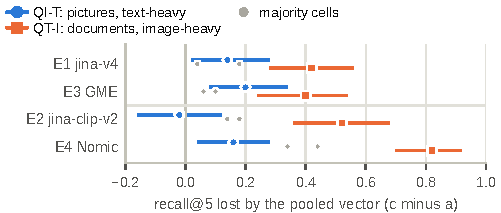
\includegraphics[width=\columnwidth]{fig_searcher_col.pdf}
\caption{The loss on queries that a model wrote as a simulated searcher: recall@5 of \rep{c} minus \rep{a} with creator-clustered 95 percent intervals, 50 queries per cell from 100 confirmation-set folders. The registered tests are the E1 rows.}
\label{fig:searcher}
\end{figure}

\section{A mixed folder is two clusters}
\label{sec:mechanism}

If a folder's images and texts sit in different regions of the space, their mean sits in neither, and a query of the smaller group is far from it. The published remedy for the modality gap is per-modality mean-centering \citep{li2025grclip}. We registered on the main set that the centered pooled centroid \rep{ac}, still one vector per folder, recovers more than half of what \rep{c} recovers.

Centering closes most of the global gap and leaves each folder split. On the main set's evaluation split the distance between the mean image-input vector and the mean text-input vector falls from 0.361 to 0.072. Before centering, a cross-modality pair in the same folder has cosine 0.524, against 0.770 and 0.722 within a modality, and after centering 0.205 against 0.568 and 0.462. The same separation holds on the confirmation set under all four encoders. The gap there runs from 0.369 under E3 to 1.095 under E4, and under E4 a folder's images and texts are close to orthogonal (cross cosine 0.066 against 0.917 and 0.698 within a modality).

The test died. On the main set \rep{ac} recovers 49 percent of \rep{c}'s gain over \rep{a} in both minority cells, and on the confirmation set 8 to 62 percent across encoders and cells. A balanced single vector, the mean of the two group means, recovers 92 to 93 percent of the minority loss on the main set and pays for it in the majority cells, at 0.071 and 0.113 below \rep{c}. No single vector we tried held both the minority and the majority (Section~\ref{sec:remedy}).

\section{Heterogeneity, and modality as its usual source}
\label{sec:hetero}

A pooled mean dilutes any minority, and a folder's minority modality is one kind of minority. On natural folders the two cannot be told apart, because label-blind clustering of a folder's files recovers the modality partition. On the main set the blind clusters are 0.88 to 0.99 pure by input group. We registered on the main set that \rep{c} beats blind $k$-means at its own budget in both minority cells, and the test died, at $+0.000$ \ci{-0.005}{+0.006} and $+0.001$ \ci{-0.005}{+0.006}. At a fixed 2 KiB the same holds on both sources under E1. Per-label $k$-means minus blind $k$-means is $-0.002$ \ci{-0.004}{-0.000} over all confirmation queries and $-0.003$ \ci{-0.011}{+0.004} on the GitHub minority files (post hoc). The label does not replace the clustering. It fixes how the budget is split across the groups. With the same number of centroids in every folder, the labels move recall from the majority image files to the minority files at one per label under E1 to E3. From three per label up they are within 0.015 of blind centroids in every cell under all four encoders. Under E4 without centering, blind centroids at the labelled count never come within the margin of searching every file, while four per label do (Section~\ref{sec:remedy}). From three per label up blind $k$-means is about as good a default, except under E4 without centering.

A control planted the files of another single-group record into single-group hosts of the main set, at a fraction drawn uniformly from $[0.2, 0.5)$, once from the host's input group and once from the other. On the 10 hosts with guest queries in both settings, the loss of \rep{a} against \rep{d} on guest queries is 0.763 for cross-modal guests and 0.583 for same-modal ones, a difference of $+0.180$ \ci{+0.021}{+0.345}, so the registered test survived, on few hosts. Most of the loss is present with no modality difference, and replacing every image by the embedding of its caption leaves the pooled vector's loss in place (Section~\ref{sec:abstracts}). One vector cannot cover a heterogeneous folder, modality is the usual source of heterogeneity in these folders, and the modality gap adds to the loss.

\section{Text queries}
\label{sec:nlq}

The same vectors can answer a text query that is not a file. With the Zenodo record's title as the query (2,597 queries) and the record's directory as the relevant folder, the registered test that the pooled centroid loses to \rep{c} on image-heavy directories under E1 survived at $+0.182$ \ci{+0.158}{+0.206}. There the loss is $+0.218$ to $+0.548$ under the other three encoders, and $+0.189$ to $+0.555$ under all four with the title and description as the query (2,399 queries). Over all titles under E1, BM25 over each folder's file names, image captions and text heads reaches recall@5 0.746, against 0.792 for \rep{c} and 0.658 for \rep{a}, and file names alone reach 0.373.

\section{Validity checks}
\label{sec:validity}

Two features of the corpus could inflate the loss. Files of one record often share a naming pattern or come in pairs, such as a figure and its PDF, and such siblings can make a folder easy to find from any one of its files. Some creators deposited many records, so intervals that treat folders as independent may be too narrow. We tested both on the confirmation set under all four encoders (Table~\ref{tab:validity}), with the tests fixed before any loss on the new subsets was computed.

\begin{table}[t]
\caption{The loss under creator clustering and on the clean subset (confirmation set): recall@5 of \rep{c} minus \rep{a} in the minority cells, with 95 percent intervals from the directory bootstrap and from resampling creator families. The clean subset holds 750 P1 and 877 P2 queries, and its intervals are creator-clustered.}
\label{tab:validity}
\setlength{\tabcolsep}{3pt}
\resizebox{\columnwidth}{!}{%
\begin{tabular}{llrllrl}
\toprule
& & \multicolumn{3}{c}{All queries} & \multicolumn{2}{c}{Clean subset} \\
\cmidrule(lr){3-5}\cmidrule(lr){6-7}
Encoder & Cell & \rep{c} $-$ \rep{a} & Directories & Creators & \rep{c} $-$ \rep{a} & Creators \\
\midrule
E1 & P1 & $+0.253$ & \ci{+0.214}{+0.294} & \ci{+0.202}{+0.303} & $+0.128$ & \ci{+0.074}{+0.180} \\
 & P2 & $+0.169$ & \ci{+0.136}{+0.200} & \ci{+0.119}{+0.225} & $+0.172$ & \ci{+0.126}{+0.222} \\
E2 & P1 & $+0.500$ & \ci{+0.462}{+0.538} & \ci{+0.456}{+0.544} & $+0.323$ & \ci{+0.264}{+0.383} \\
 & P2 & $+0.348$ & \ci{+0.312}{+0.386} & \ci{+0.255}{+0.446} & $+0.298$ & \ci{+0.247}{+0.343} \\
E3 & P1 & $+0.205$ & \ci{+0.164}{+0.244} & \ci{+0.152}{+0.260} & $+0.095$ & \ci{+0.038}{+0.150} \\
 & P2 & $+0.158$ & \ci{+0.125}{+0.188} & \ci{+0.111}{+0.209} & $+0.163$ & \ci{+0.115}{+0.218} \\
E4 & P1 & $+0.442$ & \ci{+0.398}{+0.482} & \ci{+0.396}{+0.482} & $+0.248$ & \ci{+0.187}{+0.304} \\
 & P2 & $+0.433$ & \ci{+0.396}{+0.470} & \ci{+0.317}{+0.549} & $+0.391$ & \ci{+0.331}{+0.444} \\
\bottomrule
\end{tabular}}
\end{table}

\paragraph{File names.} A router that sees only file names scores each folder by the best TF-IDF cosine, over character 3- and 4-grams of the lowercased base name, between the query file's name and the names of the folder's files. It reaches recall@5 0.700 over all queries, against 0.692 for the pooled E1 vector (Table~\ref{tab:cells}). No encoder here reads a file name, but files whose names give their folder away may resemble their siblings in content as well. Fused with the name ranking by reciprocal rank fusion ($k = 60$, post hoc), the loss keeps about two fifths of its size under the two vision-language embedders and most of it under the dual towers. Under E1 it is $+0.104$ \ci{+0.067}{+0.144} in P1 and $+0.067$ \ci{+0.041}{+0.097} in P2 (creator-clustered).

\paragraph{The clean subset.} A query is clean if the name router misses its folder and its folder holds no other file with the same stem and a different extension. Its record must also lie outside four digitization series, which a count of P2 queries singled out before any loss was computed on them. The registered test required \rep{c} minus \rep{a} of at least $+0.05$ on clean queries, with a creator-clustered interval above zero, in P1 and P2 under E1 and E3. It survived, and the same holds under E2 and E4. On clean queries the image-query loss is about half the loss over all queries under E1, E3 and E4, and the text-query loss changes little.

\paragraph{Creators.} A record's family is its first creator, lowercased. The 2,597 records come from 1,814 families, and about 47 effective families stand behind the 2,146 P2 queries. The registered test required the interval from resampling families to lie above zero in P1 and P2 under each encoder, and it survived under all four. Weighting every family equally gives $+0.133$ \ci{+0.103}{+0.163} and $+0.137$ \ci{+0.110}{+0.164} under E1, and on the clean subset $+0.059$ \ci{+0.025}{+0.094} and $+0.115$ \ci{+0.083}{+0.148} ($+0.056$ \ci{+0.023}{+0.090} and $+0.096$ \ci{+0.060}{+0.132} under E3). For image queries that is the most conservative reading the study offers, and under it the image-query loss under the vision-language embedders is about 0.06, with intervals that reach 0.02. Read as the GitHub draws are read (Section~\ref{sec:github}), with the query's folder holding another file of its input group and families weighted equally, the loss is $+0.266$ \ci{+0.224}{+0.313} and $+0.239$ \ci{+0.199}{+0.276}, and query-weighted $+0.324$ and $+0.218$ (95 percent intervals, post hoc). About a fifth of the P1 and P2 queries are lone files with no sibling of their group in the folder, and they pull the family-weighted estimates over all of P1 and P2 down.

\paragraph{A second implementation.} An agent wrote a second evaluation from a written specification without reading the first one's code. On the E1 vectors it gives the same rank for every one of the 17,140 queries in rows \rep{a}, \rep{c} and \rep{d}.

\section{A second source: GitHub directories}
\label{sec:github}

The Zenodo pool was selected for records that hold both an image and a document, all from one repository. The second source is the directories of public GitHub repositories, folders that people built for their own work. Days from 2016 to 2025 were drawn at random. For each day the pool holds the repositories created that day with at least five stars that are not forks, are at most 200 MB and carry one of nine permissive licences, as the search API returns them \citep{github2026search}. A folder is a directory of the default branch at any depth with its direct children, outside hidden, vendored and dependency directories, under the file rules of the Zenodo sets. A directory with 3 to 100 kept files is eligible, and it is mixed if it keeps an image and at least one other file. From each repository read, the scored set takes at most two mixed and two other eligible directories at random.

The readings are stricter. The minority cells keep only the queries whose folder still holds another file of the query's input group (P1s, P2s), since a lone image among texts has no sibling to be found through. The owner, the account that holds the repository, takes the place of the creator. A test is the mean over owners of the owner's mean, with intervals from 10,000 resamples of owners, and a test with fewer than 100 owners is inconclusive. A loss is confirmed if the lower end of its interval is at least $+0.05$, a smallest effect of interest fixed in advance \citep{lakens2018equivalence}. Primary tests are read on 98.33 percent intervals (Bonferroni over three).

\begin{table}[t]
\caption{The registered tests on GitHub directories: owner-weighted \rep{c} minus \rep{a} in P1s and P2s and \rep{c} minus \rep{d} where \rep{c} is a strict compression, with the number of owners and, below, the 98.33 percent interval from 10,000 resamples of owners. Fewer than 100 owners is inconclusive.}
\label{tab:github}
\setlength{\tabcolsep}{3pt}
\small
\begin{tabular}{llll}
\toprule
Draw, enc. & P1s: \rep{c} $-$ \rep{a} & P2s: \rep{c} $-$ \rep{a} & \rep{c} $-$ \rep{d} \\
\midrule
G1, E1 & $+0.193$ (86) & $+0.166$ (98) & $-0.002$ (512) \\
 & \ci{+0.099}{+0.295} & \ci{+0.080}{+0.260} & \ci{-0.014}{+0.008} \\
G1, E4 & $+0.460$ (86) & $+0.408$ (98) & $-0.002$ (512) \\
 & \ci{+0.347}{+0.574} & \ci{+0.303}{+0.517} & \ci{-0.011}{+0.007} \\
G1, E2 & $+0.471$ (86) & $+0.301$ (98) & $+0.003$ (512) \\
 & \ci{+0.357}{+0.585} & \ci{+0.204}{+0.401} & \ci{-0.005}{+0.011} \\
G2, E1 & $+0.210$ (172) & $+0.196$ (197) & $-0.002$ (918) \\
 & \ci{+0.144}{+0.279} & \ci{+0.133}{+0.260} & \ci{-0.010}{+0.006} \\
Pooled, E1 & $+0.205$ (258) & $+0.186$ (294) & $-0.002$ (1,425) \\
 & \ci{+0.152}{+0.263} & \ci{+0.135}{+0.238} & \ci{-0.008}{+0.005} \\
\bottomrule
\end{tabular}
\end{table}

\paragraph{Two draws.} The first draw, G1, holds 1,600 directories (1,000 mixed) of 1,053 owners, with 7,372 evaluation queries. Under E1, \rep{c} minus \rep{a} is $+0.193$ in P1s and $+0.166$ in P2s (Table~\ref{tab:github}). Both lower ends are above $+0.05$, but the cells hold 86 and 98 owners, so the test is inconclusive, and the rule was not relaxed. The second draw, G2, was registered after G1's table was read and drawn under the same rules from 8,307 repositories that G1 had not read. It holds 2,600 directories of 1,826 owners, with twice G1's mixed directories (2,000), and 12,951 evaluation queries. There the loss is $+0.210$ from 172 owners and $+0.196$ from 197, confirmed in both cells, and on the clean subset it is $+0.180$ and $+0.209$. Where \rep{c} strictly compresses its folder it is not inferior to \rep{d} on either draw. With commit subjects as written queries on image-heavy directories the loss is confirmed on G2 ($+0.117$ \ci{+0.065}{+0.169}, 138 owners) and inconclusive on G1 ($+0.010$).

\paragraph{The size of the loss.} Pooled over the two draws, an owner in both counted once, the loss is $+0.205$ and $+0.186$ from 258 and 294 owners. Read the same way, the Zenodo loss under E1 is $+0.266$ and $+0.239$ (Section~\ref{sec:validity}), so the GitHub loss is somewhat smaller. On all of P1 and P2, lone files included, it is $+0.069$ and $+0.071$ on G1 and $+0.055$ and $+0.095$ on G2, and more than half of G1's P1 queries are lone images among texts.

\paragraph{At the natural mix.} Mixed directories are rare. Of the 35,970 eligible directories of the repositories G1 read, 1,501 are mixed (4.2 percent), and 5.0 percent of G2's are. The scored sets over-sample them on purpose. Over all evaluation queries, owner-weighted and pooled (post hoc, as is the rest of this paragraph), \rep{c} minus \rep{a} is $+0.019$ \ci{+0.012}{+0.026}. It is $+0.030$ \ci{+0.022}{+0.039} on the queries of mixed directories and $-0.017$ \ci{-0.026}{-0.008} on the queries of the others, where the representatives lose a little to the mean. Weighted to the eligible share of mixed directories, directory-weighted within each stratum, the net is $-0.014$ \ci{-0.022}{-0.005} (post hoc). Those candidates are still the scored sets' folders, which over-sample mixed ones. Natural-mix candidates take every folder of a draw that is not mixed and add mixed ones in their eligible share, about 630 in all. Against them the net is $-0.006$ \ci{-0.012}{-0.000}.

\paragraph{Representatives for mixed folders only.} A file system can tell a mixed folder by its file types alone. We tested that policy, registered before it ran on the same draws (post hoc). It keeps \rep{c} for a folder that holds an image and another file and \rep{a} for the rest. At the natural mix, with the candidates above and 98.33 percent intervals, it gains $+0.143$ \ci{+0.094}{+0.197} in P1s and $+0.180$ \ci{+0.134}{+0.228} in P2s against \rep{a}, where \rep{c} for every folder gains $+0.164$ and $+0.192$. Over all directories it is level with the mean, $+0.001$ \ci{+0.0004}{+0.002}, not inferior by a margin of 0.005. Against \rep{c} for every folder it is $+0.007$ \ci{-0.0001}{+0.015} over all directories, so the registered test that it is better failed by its bound. The verdicts hold for the registered candidate set of about 630 folders. With the scored sets' candidates the policy is $-0.004$ \ci{-0.009}{+0.001} over all directories, just outside the margin.

\section{A written folder abstract}
\label{sec:abstracts}

RAPTOR and OpenViking represent a group of items by a summary that a language model writes, and embed the summary. We tested that design on the confirmation set under E1 and E3. Qwen3-VL-8B-Instruct captioned every image and wrote one abstract per folder, of at most 4,000 characters, from the captions, the first 500 tokens of every text and the files' name words, asked to cover every kind of file. The queries are the record titles and one-sentence descriptions of single images, written by Pixtral-12B, a model from outside the Qwen family. On the descriptions of minority images the abstract does no better than the pooled vector. Under E1 both reach recall@5 0.490 against 0.781 for \rep{c}, and under E3 the abstract reaches 0.404 against 0.747. On the titles of image-heavy folders the abstract is level with \rep{c} under E1 and below it under E3, and added to \rep{c} it gains $+0.025$ and $+0.010$ over all titles. Replacing every image by the embedding of its caption does not help the pooled vector, and per-group representatives still recover the loss in that all-text space.

\section{What fits in a folder's bytes}
\label{sec:remedy}

\paragraph{No single vector.} We searched for the most compact folder vector that keeps the minority without losing the majority, choosing every parameter on the calibration queries of the main set and reading the test on its 18,742 evaluation queries. The single vectors were weighted pooling of the two input groups' means, uncentered and centered, and the same after a linear alignment of the image group (Procrustes, ridge regression, CORAL). The registered test, that the configuration selected on the calibration queries does not come within 0.02 of \rep{c} in all four cells, survived, and the same holds post hoc for all 40 distinct single vectors scored. The binding cell is M2, where every one is at least 0.042 below \rep{c} on text queries in text-heavy folders.

\paragraph{How many vectors.} We varied the budget on the confirmation set under all four encoders, with the reading registered before the new rows ran, on a set already read (post hoc). The rows keep $k$ centroids per label for $k$ from 1 to 5 ($k = 3$ is \rep{c}), $K$ blind centroids for $K$ from 2 to 6 and 8, or as many blind centroids as the labelled rows keep, each uncentered and centered. A budget qualifies when the lower end of the interval of its difference from \rep{d} is at or above $-0.02$ over all queries and in all four cells. Four per label (6.02 vectors per folder) is the smallest labelled budget that qualifies under all four encoders, uncentered or centered. Three per label qualifies uncentered under E3 only, and falls just below the margin in M1 under E1 ($-0.021$), in M2 under E2 ($-0.025$) and in three cells under E4, down to $-0.024$. Uncentered blind centroids never qualify under E4, and centered ones need eight. Two blind centered clusters, a post hoc pick from a grid on the main set, passed their registered test against \rep{c} under E1 by the rule and fall short of the margin against \rep{d} under every encoder. On the second GitHub draw under E1 no budget qualifies in the minority cells, where the intervals resample owners and are wider.

\paragraph{The budget in bytes.} \rep{c} uses 5.2 vectors per folder on the confirmation set. We stored every vector of \rep{a}, \rep{c} and \rep{d} in five formats and scored the confirmation queries again under the four encoders (Table~\ref{tab:bytes}). The formats are float32, float16, one byte per dimension (the vector divided by its largest absolute entry, multiplied by 127 and rounded), four bits (the same with 7) and one bit (the sign). A stored vector is decoded and normalised before scoring, and the query stays in float32, since it is embedded at search time \citep{shakir2024quantization}. One byte per dimension costs at most 0.001 against float32 in any cell. At one bit \rep{c} passes the registered rule against \rep{d} under E1 and E3 and fails under the two dual towers, and it still beats the pooled centroid in float32 in the minority cells, by $+0.172$ to $+0.503$. At 8 KiB every folder's \rep{c} fits under every encoder, at one bit under E1 and E3 and at four bits under E2 and E4, at most 0.007 below float32 over all queries and 0.012 in any cell. The flat walk grows with the folder, to 491,520 bytes in float32 under E1 for 60 files.

\begin{table}[t]
\caption{\rep{c} in a metadata field of fixed size (confirmation set). For each budget per folder, the most precise format in which every folder's \rep{c} fits and its recall@5 over all queries, in P1 and in P2. The formats f32 and f16 are single and half precision, int8 is one byte per dimension, int4 four bits and bin one bit. None means that no format fits. The last two rows give \rep{c} and \rep{a} in float32 without a budget.}
\label{tab:bytes}
\setlength{\tabcolsep}{2.9pt}
\small
\begin{tabular}{llrrrlrrr}
\toprule
& \multicolumn{4}{c}{E1 jina-embeddings-v4} & \multicolumn{4}{c}{E3 gme-Qwen2-VL-2B} \\
\cmidrule(lr){2-5}\cmidrule(lr){6-9}
Budget & format & all & P1 & P2 & format & all & P1 & P2 \\
\midrule
2 KiB & none & & & & none & & & \\
4 KiB & bin & 0.796 & 0.676 & 0.543 & bin & 0.810 & 0.743 & 0.558 \\
8 KiB & bin & 0.796 & 0.676 & 0.543 & bin & 0.810 & 0.743 & 0.558 \\
\rep{c}, no budget & f32 & 0.796 & 0.674 & 0.539 & f32 & 0.811 & 0.741 & 0.544 \\
\rep{a}, no budget & f32 & 0.692 & 0.421 & 0.370 & f32 & 0.716 & 0.536 & 0.386 \\
\midrule
& \multicolumn{4}{c}{E2 jina-clip-v2} & \multicolumn{4}{c}{E4 Nomic Embed v1.5} \\
\cmidrule(lr){2-5}\cmidrule(lr){6-9}
Budget & format & all & P1 & P2 & format & all & P1 & P2 \\
\midrule
2 KiB & bin & 0.675 & 0.558 & 0.376 & bin & 0.648 & 0.377 & 0.431 \\
4 KiB & bin & 0.675 & 0.558 & 0.376 & bin & 0.648 & 0.377 & 0.431 \\
8 KiB & int4 & 0.676 & 0.554 & 0.379 & int4 & 0.692 & 0.443 & 0.441 \\
\rep{c}, no budget & f32 & 0.683 & 0.555 & 0.383 & f32 & 0.693 & 0.448 & 0.438 \\
\rep{a}, no budget & f32 & 0.457 & 0.055 & 0.035 & f32 & 0.397 & 0.006 & 0.005 \\
\bottomrule
\end{tabular}
\end{table}

\paragraph{Smaller budgets.} At 2 KiB, the user-metadata allowance of Amazon S3 and half an ext4 block, a folder holds eight one-bit vectors under E1. On the GitHub folders that do not fit whole we registered three comparisons. A sample of the folder's own files dealt to its kinds beats the mean on the minority files, by $+0.258$ \ci{+0.198}{+0.321} pooled over the two draws, and beats a sample that ignores the kinds by $+0.103$ \ci{+0.067}{+0.142} (98.33 percent intervals). Blind $k$-means centroids beat it over all queries, by 0.042 on G1 and 0.052 on G2.


\paragraph{On a file system.} Written to ext4 as an extended attribute of the directory, a summary of 2,048 or 4,000 bytes costs 1.20 blocks per summary read on a cold descent, against 2.04 for a sidecar file. Git and a plain copy drop the attribute, and times were not measured.

\section{Walking a repository tree}
\label{sec:tree}

A summary on each folder can guide a reader down a tree. We built that walk on 261 whole GitHub repositories (33,092 files in 8,587 directories), each directory with a summary of its subtree and one of its own files, the held-out query removed. From the root the reader scores staying by the directory's own summary and each child by its subtree summary, and stops when staying wins. A flat reader reads every directory's own summary. A summary that merges exactly up the tree keeps a fixed share of its slots per kind (fsample). The minority cell holds the queries whose input group is under half of the repository's other files and whose directory holds a sibling of their group. At 2 KiB under E1, on 98.33 percent intervals, the per-kind sample walks to the minority files $+0.024$ \ci{-0.022}{+0.073} more often than the mean, which is inconclusive, and $+0.064$ \ci{+0.028}{+0.104} more often than the uniform sample, so the kinds matter. The walk reads 0.39 of the summaries the flat reader reads and finds the target 0.069 \ci{0.054}{0.086} less often, inferior by its registered rule. Over all queries the mean is the best summary for the walk at 2 and 8 KiB (Table~\ref{tab:tree}). In the flat read it is also ahead of every file at one bit, over all queries and on the minority files, which we have not explained. At 8 KiB the per-kind sample walks to the minority files $+0.067$ \ci{+0.031}{+0.103} more often than the mean.

\begin{table}[t]
\caption{Success on 261 repository trees under E1, owner-weighted. Walk: the reader stops in the target directory. Flat: the target ranks first among the tree's directories. Min.: the repository-level minority cell. Every file at one bit has no budget, and file names use no vector.}
\label{tab:tree}
\setlength{\tabcolsep}{3.4pt}
\small
\begin{tabular}{lrrrrrr}
\toprule
& \multicolumn{4}{c}{2 KiB} & \multicolumn{2}{c}{8 KiB} \\
\cmidrule(lr){2-5}\cmidrule(lr){6-7}
& walk & min. & flat & min. & walk & min. \\
\midrule
mean & 0.630 & 0.686 & 0.671 & 0.782 & 0.630 & 0.686 \\
usample & 0.542 & 0.646 & 0.599 & 0.745 & 0.614 & 0.731 \\
fsample & 0.528 & 0.710 & 0.597 & 0.745 & 0.605 & 0.753 \\
sample & 0.537 & 0.723 & 0.599 & 0.746 & 0.613 & 0.753 \\
every file, one bit & 0.625 & 0.753 & 0.625 & 0.753 & 0.625 & 0.753 \\
file names & 0.477 & 0.649 & 0.478 & 0.655 & & \\
\bottomrule
\end{tabular}
\end{table}

\section{Discussion}

\paragraph{The rule for a router or an agent's memory.} Consider a system that summarises each folder, collection or source by one vector, such as a source router for retrieval-augmented generation \citep{dhasade2026ragroute}, an agent's directory-shaped memory or a folder-level file search. It can keep the mean where a folder does not mix images with other files, and it should keep a few representatives per kind where it does. A file system tells the two apart by file type without embedding anything. On GitHub directories that policy kept most of the minority gain and was level with the mean over all directories at the natural mix (Section~\ref{sec:github}, post hoc). Whether it also beats representatives for every folder was tested and not shown. Where a folder mixes, the mean loses 0.16 to 0.25 recall@5 on the minority files under two vision-language embedders, more under two dual towers, and 0.06 to 0.12 with creators weighted equally on queries whose names do not give the folder away (Section~\ref{sec:validity}). On queries that a model wrote as a simulated searcher it loses 0.14 on pictures in text-heavy folders and 0.42 on documents in image-heavy ones under the first embedder. With fewer collections competing the loss is smaller, 0.01 to 0.05 among 10 and 0.11 to 0.16 among 100 (Section~\ref{sec:loss}, post hoc), so a router that chooses among a few sources loses little of it. On the confirmation set four representatives per label were not inferior to searching every file under all four encoders (post hoc), and every folder's three per label fit in 8 KiB at one or four bits per dimension. The mean remains the better summary for the inner nodes of a tree over all queries.

\paragraph{Limitations.} \emph{Setting.} No experiment routes through file-system metadata. With every file vector in memory, a flat approximate index over the files matched a two-stage search through \rep{c} on the main set, so the case for a folder vector rests on the setting where the file vectors have not been read. The storage study counts blocks on one kernel with random bytes of the right sizes, and no times were measured. Each query faced 400 to 2,808 candidate folders, and smaller candidate sets were simulated by drawing folders at random, which may differ from the candidates a real router sees. \emph{Sources.} The Zenodo folders are researchers' deposits of 3 to 60 files, whose images are mostly figures, from a pool selected for mixed records. The GitHub directories come from repositories with at least five stars and a permissive licence. The natural-mix estimates reweight strata that take at most two directories per stratum and repository. The test of the mixed-only policy was registered on draws the study had already read. Personal working directories, mailboxes and agent memories were not measured. \emph{Queries.} Relevance is structural, and the one relevant folder of a held-out file is its own. Titles, descriptions and commit subjects are other people's words. The searcher queries were written by a model from what a person would see, cover 100 folders of one set and may be more specific than a person's. No person wrote queries for this study. \emph{Encoders.} The two vision-language embedders share a lineage (Qwen2.5-VL-3B and Qwen2-VL-2B), and both towers passed the pilot check weakly. G2 and the trees were read under E1 alone, and the searcher-query tests were registered under E1. \emph{Budgets and margins.} The seed was varied on the confirmation set only, and the budget there and, under E1, on the second GitHub draw, where no budget meets the margin in the minority cells. The margins (0.02 against the flat walk, 0.05 as the smallest loss of interest on GitHub, 0.005 for the mixed-only policy) were fixed in the briefs without an argument from the setting, and the non-inferiority readings on the Zenodo sets are query-weighted. \emph{What was not tried.} Learned fusion of names and vectors, trained pooling networks, corrections of the gap that retrain the encoder and late-interaction encoders.

\section{Conclusion}

Under the first embedder, on GitHub directories that do not mix media, the mean of a folder's embeddings did at least as well as a few representatives (post hoc). Where a folder mixes images and texts, the mean misses the files that differ from the rest of the folder, by about a fifth of recall@5 under vision-language embedders and more under dual towers. Under the first embedder it also misses them on queries that a model wrote as a simulated searcher. Four representatives per file type were not inferior to searching every file, in every cell under all four encoders on the confirmation set (post hoc). Three fit every folder's metadata in 8 KiB at a further cost of at most 0.012 in any cell. Keeping representatives only for the folders that mix, chosen by file type, was level with the mean over all GitHub directories at their natural mix (post hoc). It was not shown to beat representatives for every folder.

\section*{Use of AI}

The authors used AI assistants (Claude, Anthropic; Gemini, Google) throughout this work, for writing, coding, analysis and review. The study's sessions were working sessions in which the authors directed such an assistant, the second implementation of Section~\ref{sec:validity} was written by one, and ``agent'' in the text means such an assistant. The rounds of review that the text mentions were done by such assistants. Models also produced study materials. Qwen3-VL-8B-Instruct wrote the image captions and folder abstracts of Section~\ref{sec:abstracts}, and Pixtral-12B wrote the image descriptions used there as queries. Claude Opus 5.5 wrote the searcher queries of Section~\ref{sec:searcher}, as a simulated searcher that was told nothing about the study. No person wrote queries for this study. The authors conceived and directed the study and take full responsibility for its content.

\bibliographystyle{ACM-Reference-Format}
\bibliography{refs}

\end{document}
